\documentclass[14pt, a4paper]{extreport}
\usepackage{susu}

% ====================================================================================================
\begin{document}

\author{Савонин~М.В.}
\group{211}
\task{3}
\maketitle

% ====================================================================================================
\chapter{Задание}

\begin{enumerate}

	\item
	Привести описание и схему алгоритма Ву для растрового представления линии.

	\item
	Разработать подпрограмму для рисования линии (аналог процедуры line из графической библиотеки). Аргументы подпрограммы – координаты 				начальной и конечной точек. При реализации подпрограммы использовать для рисования только процедуру putpixel. Для определения текущего 			цвета рисования использовать функцию getcolor.

	\item
	Разработать подпрограмму для рисования правильной звезды. Аргументы подпрограммы – координаты центра, радиус описанной окружности и 			число вершин. При создании контура звезды использовать собственную подпрограмму рисования линии. Для закраски фигуры использовать 				процедуру floodfill.

	\item
	Написать программу для тестирования разработанных подпрограмм. Интерфейс программы должен содержать следующие элементы управления:
	\begin{itemize}
		\item увеличение/уменьшение числа вершин;
		\item увеличение/уменьшение размера (радиуса описанной окружности);
		\item сохранение результата в файл;
		\item выход из программы.
	\end{itemize}

\end{enumerate}

% ====================================================================================================
\chapter{Математическая модель}

Пусть $x_1$, $y_1$, $x_2$, $y_2$ -- соответственно координаты первой и второй точки.
При рисовании линии цвет задан изначально $col_0$, $col_1$ и $col_2$ в формате RGB и будем говорить что он равет col, а координаты простовляемого пикселя x и y.\\
Рисование линии:
$$ dx = |x_2-x_1| . $$
$$ dy = |y_2-y_1| . $$
$$ err = 0 . $$
$$ derr = 200 . $$
Если dx не равен 0, то:
$$ derr = 200*dy/dx . $$
Если Изменение ошибки derr < 200, то: \\

Если $x_1$ > $x_2$, то меняем точки местами.
$$ y = y_1 . $$

Если dy = 0 то и d = 0, иначе:
$$ d = \frac{y_2-y_1}{dy} . $$

Закрашиваем пиксель в начальной точке $x_1$, $y_1$ цвета col.

Потом перебераем все значения x от $x_1$ до $x_2$:

Ставим пиксель в координах x y и с цветом (200-err)*col/200 и в координах x y+d и с цветом err*col/200.
$$ err = err+derr . $$

Если err $\geq$ 200:
$$ y = y+d. $$
$$ err = err-200. $$
Если Изменение ошибки derr $\geq$ 200, то:

Если $y_1$ > $y_2$, то меняем точки местами.
$$ x = x_1 . $$

Если dx = 0 то и d = 0, иначе:
$$ d = \frac{x_2-x_1}{dx} . $$

Закрашиваем пиксель в начальной точке $x_1$, $y_1$ цвета col.

Потом перебераем все значения y от $y_1$ до $y_2$:

Ставим пиксель в координах x y и с цветом (200-err)*col/200 и в координах x+d y и с цветом err*col/200.
$$ err = err+derr . $$

Если err $\geq$ 200:
$$ x = x+d. $$
$$ err = err-200. $$


% ====================================================================================================
\chapter{Текст программы}

\noindent Файл main.cpp
\lstinputlisting{source/main.cpp}
\pagebreak
\hrulefill

\noindent Файл task.h
\lstinputlisting{source/task.h}
\hrulefill

\noindent Файл task.cpp
\lstinputlisting{source/task.cpp}
\hrulefill

\noindent Файл control.h
\lstinputlisting{source/control.h}
\hrulefill

\noindent Файл control.cpp
\lstinputlisting{source/control.cpp}

% ====================================================================================================
\chapter{Результат работы}

\begin{figure}[h!]
	\centering
	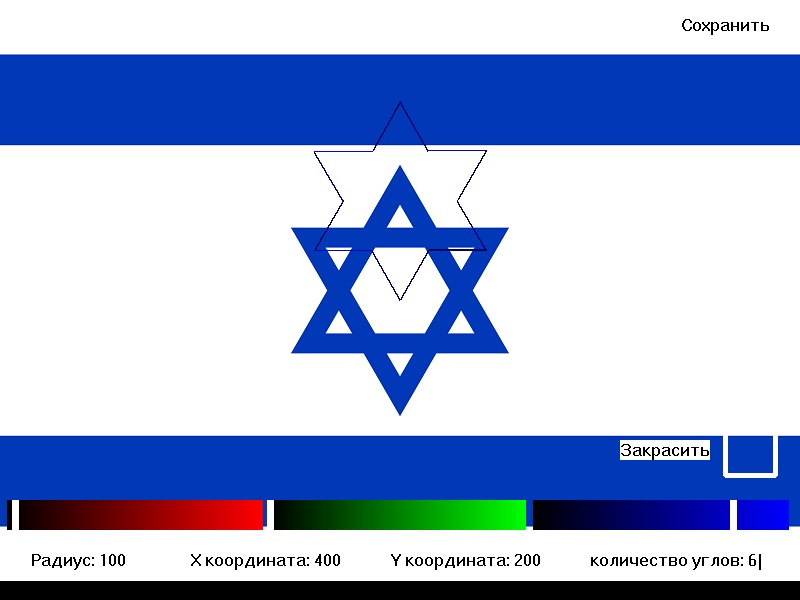
\includegraphics[width = 12cm]{image/image_1}
  \caption{Результат выполнения программы (Пример 1)}
\end{figure}

\begin{figure}[h!]
	\centering
	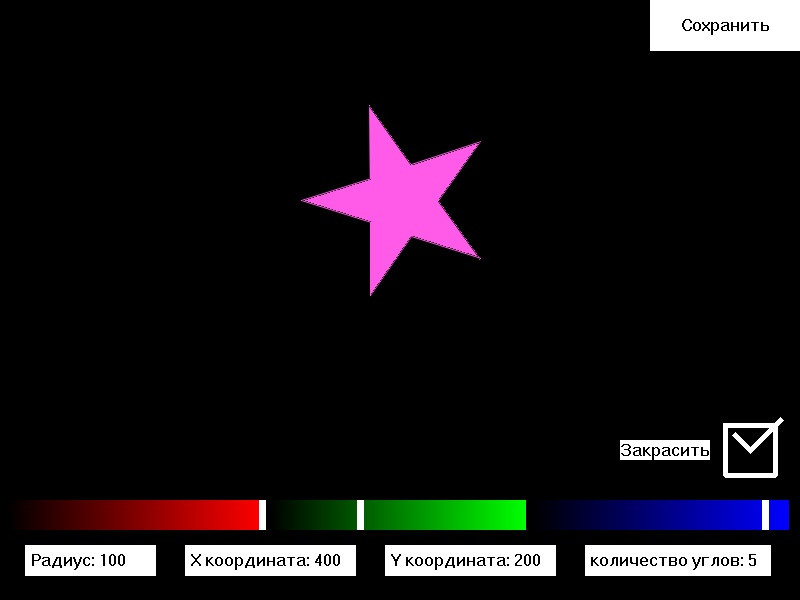
\includegraphics[width = 12cm]{image/image_2}
  \caption{Результат выполнения программы (Пример 2)}
\end{figure}

\begin{figure}[h!]
	\centering
	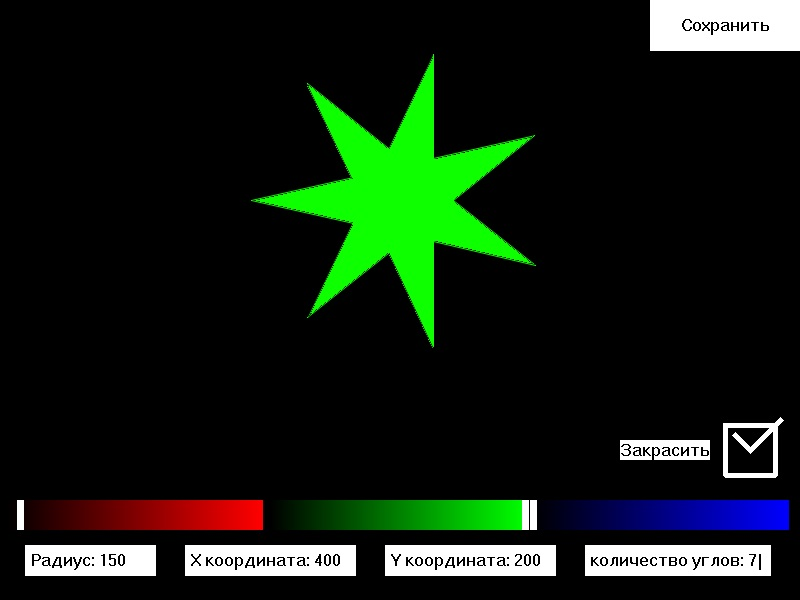
\includegraphics[width = 12cm]{image/image_3}
  \caption{Результат выполнения программы (Пример 3)}
\end{figure}

% ====================================================================================================
\end{document}